\documentclass[10pt]{article}

\usepackage[utf8]{inputenc}
\usepackage[portuges]{babel}
\usepackage{a4wide}
\usepackage{graphicx}
\usepackage[export]{adjustbox}
\usepackage[labelformat=empty]{caption}
\graphicspath{ {img/} }

\begin{document}

\title{Projeto de Laboratórios de Informática 3\\2ª Fase\\Grupo 34}
\author{Alexandre de Freitas Ferreira Pacheco A80760\and Diogo José Cruz Sobral A82523\and José Pedro Milhazes Carvalho Pinto A80741}


\date{\today}


\maketitle

\begin{figure}[h]
	\minipage{0.32\textwidth}\centering
		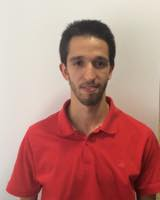
\includegraphics[scale=0.5]{A80760.png}
		\caption{A80760}
		\label{fig1:A80760}
	\endminipage\hfill
	\minipage{0.32\textwidth}\centering
		
\includegraphics[scale=0.5]{A82523.jpg}
		\caption{A82523}
		\label{fig2:A82523}
	\endminipage\hfill
	\minipage{0.32\textwidth}\centering
		
\includegraphics[scale=0.5]{A80741.jpeg}
		\caption{A80741}
		\label{fig3:A80741}
	\endminipage
\end{figure}


\begin{abstract}
		Como já foi visto, nesta unidade curricular foi-nos proposta 
	a implementação de um sistema de resposta a \textit{queries} 
	sobre um \textit{dump} da  base dados do site \emph{Stack 
	Overflow}.
		
		Era pretendido que esta segunda fase do projeto fosse
	desenvolvida em \emph{Java}. Pelo que o esperado era uma maior
	facilidade na implementação das soluções para qualquer problema 
	que surgisse e em atingir objetivos como o o encapsulamento das
	estruturas de dados e a abstração de código.
	
		Ao longo desta segunda fase do projeto não pudemos deixar 
	de notar a grande diferença, em termos de ferramentas disponíveis 
	e "comodidade", entre trabalhar em \emph{Java} e em \emph{C}.
\end{abstract}

\pagebreak

\section{Ferramentas Utilizadas} 

		À senelhança do que aconteceu na primeira fase do projeto,
	servimo-nos de uma biblioteca para efeturar o parsing dos 
	ficheiros \textit{xml}, que foi o \emph{Java SAXParser}.
	
		Por outro lado, para organizarmos as nossas estruturas de 
	dados, desta vez nem sequer considerámos implementar versões 
	nossas das estruturas, visto que o java já apresenta uma 
	API riquíssima em ferramentas para este propósito.
	
	
\section{Tipos e Estruturas de Dados}		

		De modo a conseguir responder às \textit{queries} propostas de forma eficiente, é natural
	que o mais importante é a forma como organizamos o grande volume de informação 
	presente nos \textit{dumps} disponibilizados.
		
		Primeiro, analisámos a informação contida em cada um dos ficheiros \textit{xml}
	disponibilizados por comunidade (e.g. \textit{android}, \textit{ubuntu}...) e o 
	que era pedido nas \textit{queries}, a fim de perceber quais os dados que seriam recorrentemente
	necessários.

	
\subsection{Tipos de Dados: \textit{Users} e \textit{Posts}}
	
		As entidades elementares na forma de descrever cada comunidade, 	à volta das quais
	gira a grande maioria da informação, são os \textit{users} e os 			\textit{posts}.
	
		Naturalmente, e semelhantemente ao que fizemos na 1ª fase, 
	para cada um destes objetos criámos uma classe, \texttt{MyUser} 
	e \texttt{MyPost}.
	
		Para representar as \textit{tags} bastou implementar uma 
	correspondência entre os seus nomes e \texttt{Ids}, como veremos 
	à frente.
	

\subsection{Organização dos Objetos de Posts e Users}
		Para organizar a informação utilizámos sobretudo a interface
	\emph{Map} do \textit{Java}.
	
		Organizámos os \textit{users} num \texttt{LinkedHashMap} em 
		que a chave são os \texttt{Ids}.
	
		Organizámos os \textit{posts}, tal como na primeira fase em
	duas estruturas separadas, para os poder procurar quer por data
	quer por \texttt{Id}.  Assim, ficaram num \texttt{LinkedHashMap} 
	semelhante ao dos \textit{users} e noutro \texttt{LinkedHashMap} 
	com as \texttt{LocalDate} como chave e uma lista de \textit{posts} 
	por cada data.
	
		Esta lista de \textit{posts} foi implementada numa classe 
	que definimos fazendo uso da interface \texttt{List} e um contador 
	de perguntas e respostas que é preenchido aquando do 
	\textit{loading.}
	
		A informação das \textit{tags} consiste num 
		\texttt{LinkedHashMap} cujas chaves são nomes das tags e 
		os valores são os \texttt{Ids} das mesmas.
		
	
\subsection{Outras Estruturas Auxiliares}
		
		Para além da organização essencial referida, decicidmos 
	implementar, ainda, estruturas auxiliares, que são úteis sobretudo 
	quando a resposta a determinadas \textit{queries} envolve calcular 
	um conjunto de perguntas mais respondidas ou um conjunto de 
	utilizadores com maior reputação.
	
		Estas estruturas consistem em duas listas, mais propriamente, 
	\texttt{ArrayList}. Um deles contém os \texttt{Ids} de todos os
	\textit{users} ordenados pelo número de posts que o respetivo
	\texttt{user} efetuou. O outro segue a mesma lógica, mas o 
	critério de ordenação é a reputação dos \textit{users}.
	
	
	
\pagebreak

\section{Modularização e Abstração de Dados}
		Como temos aprendido ao longo dos últimos tempos, são boas práticas as de 
	manter um código modular e abstraído do tipo de dados com que	trabalhamos.
	
	\subsection*{Encapsulamento}
	
		Em \textit{Java} é bastante fácil de encapsular os dados, 
	uma vez que a própria linguagem já tem mecanismos que facilitam 
	esta prática, como a simples declaração de variáveis de instância 
	como \texttt{private}. A fim de impossiblitar a propagação de 
	apontadores da estrutura interna da nossa comunidade, todos os
	\textit{sets} e \textit{gets} das classes que criámos trabalham 
	com clones. Os sets clonam a informação que recebem, e os gets 
	clonam a informação interna para devolver o clone.
	
	
	
	
	\subsection*{}
		A utilização das APIs do \textit{Java} tornou o código 
	bastante abstrato, visto que a qualquer momento podemos mudar, 
	por exemplo, o nosso programa para implementar os mapas num 
	\texttt{TreeMap} em vez de \texttt{LinkedHashMap} e pouco ou 
	nada termos de mudar. Este comportamento verifica-se na maior 
	parte do código.

\section{\textit{Queries}}
		Nesta secção passamos a explicar a abordagem que tomámos 
	em relação a cada uma das \textit{queries}, note-se que muitas 
	delas funcionam como na primeira fase.
	\subsection*{\textit{Query} 1 - Título e autor da pergunta}
		O procedimento que tomamos é bastante simples. 
		\begin{enumerate}
		\item Procuramos o post com o \texttt{Id} fornecido e verificamos se se trata
		 de uma pergunta. 
		\begin{enumerate}
		\item Se for uma pergunta, devolvemos o seu título e o \texttt{DisplayName} do autor 
	(procurado o \texttt{OwnerUserId} na árvore de users).
	
		\item Se for uma resposta, repetimos o ponto \textbf{1} com o \texttt{ParentId}
		do post, que será o \texttt{Id} da pergunta correspondente.
		\end{enumerate}
		\end{enumerate}
	\subsection*{\textit{Query} 2 - Top N \textit{users} com mais posts}
			Esta query toma partido da estrutura auziliar em que,
		aquando do \textit{load}, ordenamos os users pelo seu 
		número de \textit{posts}. Copia-se desta estrutura os 
		N primeiros utilizadores (ou todos, caso N seja maior
		que o tamanho desta coleção).			
	\subsection*{\textit{Query} 3 - Número de perguntas e respostas ao longo de um período}
			O \texttt{LinkedHashMap} que organiza os posts por data
		tem como chave a \texttt{LocalDate} referente a cada dia, e 
		como valor um objeto que contém uma lista de \texttt{Ids} de
		\textit{posts}, e dois contadores, que indicam quantas 
		perguntas e respostas ouve nesse dia. Tomando partido desta 
		organização:
		\begin{enumerate}
			\item Percorre-se um ciclo em que se acrescenta a cada 
		iteração um dia à \texttt{LocalDate} que corresponde ao 
		início do período.
			\item Em cada entrada do \textit{map}, soma-se ao total
		de perguntas o número de perguntas na lista de \textit{posts} 
		nessa entrada, e faz-se o mesmo para as repsostas.
			\item No fim do ciclo, devolve-se as variáveis que 
		acumularam o somatório ao longo do ciclo.
		\end{enumerate}
	\subsection*{\textit{Query} 4 - Perguntas com determinada \textit{tag} feitas num período}
		\begin{enumerate}
			\item Efetua-se um ciclo semelhante ao descrito na 
		\textit{query} 3 (no que toca ao modo de iteração).
			\item Em cada iteração, obtém-se e percorre-se a coleção 
		de \textit{posts} correspondentes a cada data.
			\item Se um \textit{post} tiver a \textit{tag} a verificar 
		o \texttt{Id} do mesmo é adicionado a uma lista resultado, a
		retornar no final.

		\end{enumerate}
			
	\subsection*{\textit{Query} 5 - Informação de um \textit{user} e os seus últimos \textit{posts}}
			Esta \textit{query} consiste em simplesmente procurar um utilizador na nossa estrutura
		e devolver a sua informação.			
		\begin{enumerate}
			\item É procurado o \textit{user} em questão.
			\item É percorrida a sua lista de \textit{posts}, e cada 
		um deles é adicionado a um \texttt{TreeSet} ordenado pela
		data de criação dos posts.
			\item Armazena-se os \texttt{Ids} dos 10 primeiros (ou 
		menos, se forem menos de 10) \textit{posts} do \textit{set} 
		referido numa lista-resultado.
			\item Retorna-se a biografia e a lista resultado 
			construída.
		\end{enumerate}
	\subsection*{\textit{Query} 6 - N respostas mais votadas ao longo de um período}
			A diferença entre os \textit{upvotes} e \textit{downvotes} de uma resposta
		equivale ao seu parâmetro \texttt{Score}, pelo que este já se encontra calculado
		a partir do momento em que o carregámos do ficheiro \textit{xml}.
			\begin{enumerate}
				\item É efetuado um ciclo semelhante aos referidos 
			nas \textit{queries} 3 e 4.
				\item Para cada data, percorre-se os \textit{posts} 
			correspondentes e adiciona-se os que forem respostas 
			a uma lista auxiliar.
				\item Esta lista de \textit{posts} é ordenada 
			segundo os \textit{scores} (recorrendo a um 
			\texttt{Comparator}), e devolve-se os \texttt{Ids} dos 
			primeiros N (ou menos, caso não hava N) \textit{posts}.
			\end{enumerate}
	\subsection*{\textit{Query} 7 - N perguntas com mais respostas ao longo de um período}
			A nossa \textit{query} 7 toma partido do atributo
		\texttt{AnswerCount} dos posts, pelo que a solução é bastante 
		semelhante à da \textit{query} 6. As únicas diferenças são 
		que os \texttt{Ids} devolvidos são de perguntas e não de 
		respostas, e que a ordenação feita na lista auxiliar 
		recorre a um \texttt{Comparator} que tem em conta o número
		de respostas em vez do \textit{score}.
	\subsection*{\textit{Query} 8 - N perguntas mais recentes com determinada \textit{tag}}
		Na \textit{query 8}, o critério que utilizámos para averiguar 
	se um título contém uma dada palavra foi o método 
	\texttt{String contains(String str)} da API do \textit{Java}.
			\begin{enumerate}
				\item São percorridos todos os posts do \textit{map} 
			que os organiza.
				\item Se um post contiver no título a palavra a 
			procurar, este é adicionado a um \texttt{TreeSet} 
			ordenado segundo um \texttt{Comparator} que ordena 
			cronologicamente os posts.
				\item Retorna-se numa lista resultado os \texttt{Ids} 
				dos N primeiros (ou menos de N, caso não existam) posts 
				do \textit{set} referido.
			\end{enumerate}
	\subsection*{\textit{Query} 9 - N perguntas mais recentes em que dois \textit{users} participaram}
	Esta é outra query em que se tira bastante partido do facto de termos em cada objeto que representa um \textit{user} uma lista com 
os \texttt{Ids} dos seus posts.

			\begin{enumerate}
				\item Cria-se um \texttt{HashMap<MyPost, Integer>} 
			auxiliar, onde se insere como chave as perguntas 
			correspondentes a cada \textit{post}.
				\item Percorre-se os \textit{posts} de um \textit{user} 
			e insere-se a pergunta correspondente 
			no \texttt{map} auxiliar, com o valor de 0.
				\item Repete-se o processo para o outro \textit{user},
			mas se uma dada pergunta já estiver no mapa, insere-se 
			com o valor 1.
				\item Para cada entrada do mapa auxiliar, se o seu 
			valor for 1, insere-se o \texttt{post} num \texttt{TreeSet}
			 ordenado cronologicamente recorrendo a um 
			 \texttt{Comparator}.
			 	\item Retornam-se os \texttt{Ids} dos N primeiros  
			 \textit{posts} deste \texttt{TreeSet}.			
			\end{enumerate}
	\subsection*{\textit{Query} 10 - Melhor resposta}
			Esta \textit{query} é relativamente simples, devido ao 			facto de no \texttt{load} registarmos em cada \textit{post} 
	post os \texttt{Ids} das suas respostas (caso seja uma pergunta).
						
			\begin{enumerate}
				\item É percorrida a lista de respostas do post dado,
			e para cada uma calcula-se uma pontuação mediante a 
			fórmula dada no enunciado.
				\item Retorna-se o \texttt{Id} da resposta para a qual 
			tenha sido observada uma maior pontuação.
			\end{enumerate}
	\subsection*{\textit{Query} 11 - N \textit{tags} mais usadas ao longo de um período pelos N \textit{users} com maior reputação}
			Esta \textit{query} faz uso de grande parte das estruturas que temos montadas.
		
			Nesta query, é criada um \texttt{HashMap} com 
		as ocorrências de cada \textit{tag}, que depois são 
		ordenadas num \texttt{TreeSet} para poderem ser devolvidas.
			É ainda importante mencionar que, na nossa interpretação 
		do que foi pedido, utilizámos os N utilizadores com maior 
		reputação de sempre (mesmo que não tenham postado nesse 
		período de tempo). No resultado da query, \texttt{Ids} de 
		tags com o mesmo número de ocorrências estão em ordem 
		crescente.		
		
			\begin{enumerate}
				\item É obtido um \texttt{ArrayList} com (no máximo) 
			N \texttt{Ids} de \textit{users}, ordenados pela sua 
			reputação através da estrutura auxiliar já mencionada, 
			criada para o efeito.
				\item A lista obtida é percorrida, os respetivos 
			\texttt{users} procurados no devido \texttt{LinkedHashMap} 
			e para cada um:
					\begin{enumerate}
						\item Obtêm-se os \textit{posts} que são 
						perguntas e foram efetuados no período de 
						tempo especificado.
						\item As \textit{tags} destes posts são 
					registadas, ou o seu número de ocorrências 
					incrementao, num \texttt{HashMap} criado para 
					este efeito.
					\end{enumerate}
				\item Preenchida a tabela, todas as suas entradas 
			são inseridas num \texttt{TreeSet} onde ficam 
			ordenadas pelo número de ocorrências.
				\item Retornam-se os \texttt{Ids} nas chaves das (no 
				máximo) N primeiras entradas do referido 
				\texttt{TreeSet}.
			\end{enumerate}
			
			
\pagebreak
\section{Interface Gráfica e modelo MVC}
	Tomámos também a liberdade de implementar uma interface 
gráfica (GUI) recorrendo à ferramenta \textit{Swing} e ao modelo
\textit{Model View Controller}, \emph{MVC}.

	Esta interface consiste numa possível tradução e síntese visual 
daquilo em que consiste este projeto: a escolha e \textit{loading} 
de uma \textit{dump} de dados, a introdução de \textit{inputs} para 
uma determinada \textit{query}, e a resposta por parte do programa.

	A implementação desta funcionalidade foi simples, mais uma vez 
devido à existência de imensas ferramentas de suporte ao \textit{Java} 
e também devido ao facto de a parte obrigatória do projeto estar 
pronta para ser utilizada como \textit{Model} do MVC simplesmente 
recorrendo à interface \texttt{TADCommunity}.

	Nota: Por uma questão de simplicidade, a nossa implementação 
da interface comporta-se de forma que as datas têm de ser 
introduzidas no formato "AAAA-DD-MM.." (i.e. "2001-01-01").

\begin{figure}[h]\centering
		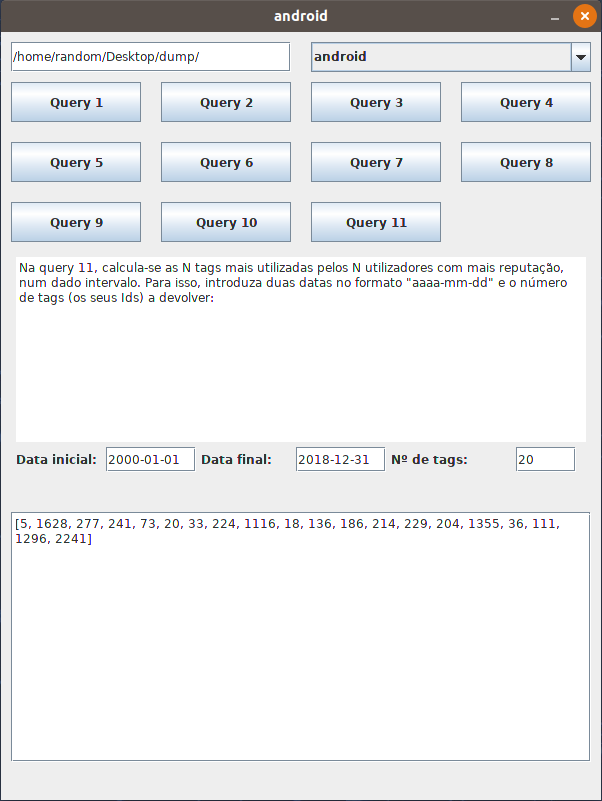
\includegraphics[scale=0.55]{gui.png}
		\caption{Exemplo de estado da interface gráfica}
		\label{fig1:gui}

\end{figure}
	
			
\pagebreak

\section{Estratégias para melhorar a Eficiência}
		Tendo em conta o grande volume de dados que nos propusemos a processar neste projeto,
	surge a necessidade de adotarmos estratégias que melhorem a eficiência das operações que
	levamos a cabo.
	
			Uma decisão que tomámos de modo a melhorar a eficiência
	foi qual implementação da interface \texttt{Map} utilizar.
	Utilizámos \texttt{LinkedHashMap} porque, uma vez que é 
	implementada utilizando listas ligadas, nunca tem espaços vazios 
	que precisem de ser atravessados numa travessia (efetuada 
	em qualquer procura por um valor, se recordarmos o funcionamento 
	de uma tabela de \textit{hash}). 
	
		A única pequena desvantagem dos
	\texttt{LinkedHashMap} em relação aos \texttt{HashMap} é na 
	criação e inserção de valores, no entanto, foi um compromisso que 
	estivemos dispostos a fazer, dado que estas estruturas são criadas 
	durante o \textit{load}.
	
		Outra forma de tornar o nosso programa mais eficiente foi, 
	durante o \texttt{load}, construir estruturas auxiliares que, 
	embora armazenassem informação que pudesse ser obtida a partir 
	das árvores de \textit{posts} e \textit{users}, e levassem a um 
	ligeiramente maior gasto de memória, eram úteis a muitas 
	\textit{queries} e poupavam imensos cálculos e travessias.
	
	
		Uma prática que procurámos ter foi a utilização de arrays 
	sempre que possível. Um bom exemplo da nossa "aproximação" aos 
	\textit{arrays} é o facto de utilizarmos \texttt{ArrayList} nas 
	estruturas que nos devolvem os N \texttt{users} com mais reputação 
	ou \texttt{posts} efetuados.




\section{Conclusão}
	Tal como na primeira fase pudemos concluir, há sempre um 
compromisso performance vs. segururança, a organização da nossas 
estruturas toma um papel central nos fatores que influenciam a 
eficiência das \textit{queries}.
	
		
	Verificámos o esperado, que era ser muito mais simples implementar 
esta solução em \textit{Java} do que em C, dado o leque de ferramentas 
(a maior parte nativa da linguagem) com que pudemos contar para 
resolver qualquer problema.

	Resta refletir sobre as duas fases do projeto e afirmar que 
muito dificilmente, se nos propusessem novamente uma tarefa 
semelhante, escolheríamos C para implementar a solução. No fundo, 
apenas uma ínfima parte dos projetos requerem virtudes que apenas 
linguagens como o C podem oferecer. Num mundo cada vez mais 
orientado aos objetos e exigente por por produtividade, é natural 
que vigore a utilização de linguagens com um maior nível de abstração.

\end{document}\grid
\grid\grid
\grid
